%%
%% This is file `sample-sigplan.tex',
%% generated with the docstrip utility.
%%
%% The original source files were:
%%
%% samples.dtx  (with options: `sigplan')
%%
%% IMPORTANT NOTICE:
%%
%% For the copyright see the source file.
%%
%% Any modified versions of this file must be renamed
%% with new filenames distinct from sample-sigplan.tex.
%%
%% For distribution of the original source see the terms
%% for copying and modification in the file samples.dtx.
%%
%% This generated file may be distributed as long as the
%% original source files, as listed above, are part of the
%% same distribution. (The sources need not necessarily be
%% in the same archive or directory.)
%%
%%
%% Commands for TeXCount
%TC:macro \cite [option:text,text]
%TC:macro \citep [option:text,text]
%TC:macro \citet [option:text,text]
%TC:envir table 0 1
%TC:envir table* 0 1
%TC:envir tabular [ignore] word
%TC:envir displaymath 0 word
%TC:envir math 0 word
%TC:envir comment 0 0
%%
%%
%% The first command in your LaTeX source must be the \documentclass command.
%%\documentclass[sigplan,nonacm]{acmart}
\documentclass[sigplan,screen,nonacm]{acmart}\settopmatter{printfolios=true,printccs=false,printacmref=false}
\graphicspath{{figure/}}
%%
%% \BibTeX command to typeset BibTeX logo in the docs
\AtBeginDocument{%
	\providecommand\BibTeX{{%
			\normalfont B\kern-0.5em{\scshape i\kern-0.25em b}\kern-0.8em\TeX}}}

%% Rights management information.  This information is sent to you
%% when you complete the rights form.  These commands have SAMPLE
%% values in them; it is your responsibility as an author to replace
%% the commands and values with those provided to you when you
%% complete the rights form.
\setcopyright{none}

%%\copyrightyear{2018}
%%\acmYear{2018}
%%\acmDOI{10.1145/1122445.1122456}

%% These commands are for a PROCEEDINGS abstract or paper.
%%\acmConference[Woodstock '18]{Woodstock '18: ACM Symposium%% on Neural
%%  Gaze Detection}{June 03--05, 2018}{Woodstock, NY}
%%\acmBooktitle{Woodstock '18: ACM Symposium on Neural Gaze Detection,
%%  June 03--05, 2018, Woodstock, NY}
%%\acmPrice{15.00}
%%\acmISBN{978-1-4503-XXXX-X/18/06}


%%
%% Submission ID.
%% Use this when submitting an article to a sponsored event. You'll
%% receive a unique submission ID from the organizers
%% of the event, and this ID should be used as the parameter to this command.
%%\acmSubmissionID{123-A56-BU3}

%%
%% The majority of ACM publications use numbered citations and
%% references.  The command \citestyle{authoryear} switches to the
%% "author year" style.
%%
%% If you are preparing content for an event
%% sponsored by ACM SIGGRAPH, you must use the "author year" style of
%% citations and references.
%% Uncommenting
%% the next command will enable that style.
%%\citestyle{acmauthoryear}

%%
%% end of the preamble, start of the body of the document source.
\begin{document}
\sloppy

%%
%% The "title" command has an optional parameter,
%% allowing the author to define a "short title" to be used in page headers.
\title{A brief study of Approximation Algorithms for 2D Packing Problem}

%%
%% The "author" command and its associated commands are used to define
%% the authors and their affiliations.
%% Of note is the shared affiliation of the first two authors, and the
%% "authornote" and "authornotemark" commands
%% used to denote shared contribution to the research.
\author{Ruiqi Gao$\dagger$}
\email{gao606@purdue.edu}
\affiliation{%
  \institution{Purdue University}
  \city{Lafayette}
  \state{Indiana}
  \country{USA}
  \postcode{47901}
}
\author{Aocheng Li$\dagger$}
\email{li3922@purdue.edu}
\affiliation{%
	\institution{Purdue University}
	\city{Lafayette}
	\state{Indiana}
	\country{USA}
	\postcode{47901}
}



%%
%% By default, the full list of authors will be used in the page
%% headers. Often, this list is too long, and will overlap
%% other information printed in the page headers. This command allows
%% the author to define a more concise list
%% of authors' names for this purpose.
%%\renewcommand{\shortauthors}{Trovato and Tobin, et al.}

%%
%% The abstract is a short summary of the work to be presented in the
%% article.
\begin{abstract}
  2D Packing (Strip Packing) problem is a 2-dimensional geometric optimization problem which a collection of rectangles are packed into a unit-width bin while the packing height is minimized. In this paper, we study a series of approximation algorithms for 2D Packing Problem and analyze their performances. First we study two intuitive approximation algorithms designed by Coffman with approximation bounds of 3 and 2.7. We further investigate a more advanced algorithm designed by Steinberg that has an approximation bound of 2. Some future investigation directions for improving performance are given in the end.
\end{abstract}
\keywords{Approximation Algorithm, 2D packing, Strip Packing}

%%
%% The code below is generated by the tool at http://dl.acm.org/ccs.cfm.
%% Please copy and paste the code instead of the example below.
%%


%%
%% Keywords. The author(s) should pick words that accurately describe
%% the work being presented. Separate the keywords with commas.



%%
%% This command processes the author and affiliation and title
%% information and builds the first part of the formatted document.
\maketitle

\section{Introduction}
<<<<<<< HEAD
2D Packing Problem is defined as follows: Given a collection of rectangles $\{R_1,R_2,R_3,\dots,R_n\}$ each with a size of $w_i\times h_i, 1\leq i\leq n$, and a bin with fixed width and infinite height, we wish to pack all the rectangles into the bin without overlapping while minimizing the total bin height\cite{baker1980orthogonal}. Without loss of generality, we can normalize bin width to be 1.\par
=======
2D Packing Problem is defined as follows: We are giving a collection of rectangles $\{R_1,R_2,R_3,\dots,R_n\}$ with width $w_i$ and height $h_i$ and a bin with fixed width and infinite height, and we need to pack all the rectangles into the bin without overlapping while minimize the total bin height\cite{baker1980orthogonal}. Without loss of generality, we can normalize the width to be 1.\par
>>>>>>> first 3 section finished
\begin{figure}[htbp]
  \centering
  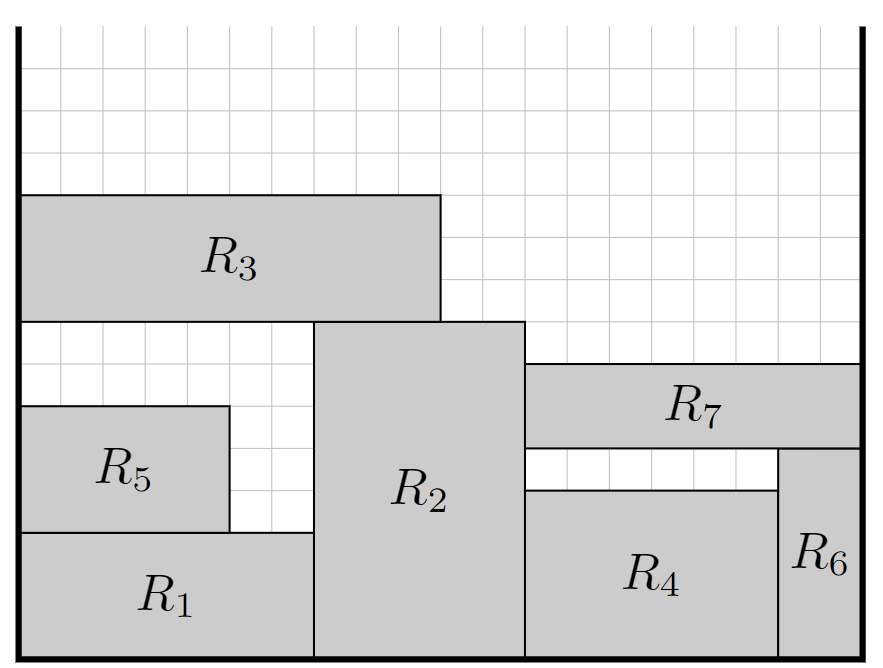
\includegraphics[scale=0.5]{2dpacking}
  \caption{2D Packing Problem}
  \label{fig:2dpacking}
\end{figure}
This problem is very important in many fields. In the transportation industry, this algorithm can be used to pack an item into containers. There is also an interesting application of this problem in main memory allocation in multi-processor programming. Basically, this problem can be adapted to most resource allocation problems with two dimension resource constraints.\par
While the description of this problem is rather simple, there is a hidden computation complexity behind this problem. Actually, this problem is NP-Complete\cite{hartmanis1982computers}, which means that there is currently no efficient deterministic algorithm to solve it. It is easy to notice that this problem is a generalized version of the one-dimension bin packing problem\cite{johnson1974worst}. Simply restrict all the rectangles' height to be 1, this problem becomes a one-dimensional bin packing problem. We can reduce the one-dimensional bin packing problem to this problem using the idea above. Because the one-dimensional bin packing problem is NP-Hard, this problem is also NP-Hard. The optimized solution to the 2D Packing problem can be easily verified, therefore the 2D Packing Problem is also in NP. Then 2D Packing Problem is NP-Complete. With $P$ $vs$ $NP$ being an open problem, we can not find an efficient algorithm for 2D Packing Problem. \par
Another interesting NP-Complete problem that is related to 2D Packing is MakeSpan minimization problem\cite{graham1966bounds} where we try to schedule jobs across multiple machines and minimize the total execution time. By simply restricting all the rectangles' height to be 1, 2D Packing Problem becomes the MakeSpan minimization problem. By finding an efficient algorithm for 2D Packing Problem, we can find an efficient solution to the MakeSpan minimization problem too. \par
We already show that 2D Packing Problem to be NP-Complete, and P vs NP remains an open problem, so we can not find an efficient algorithm to deterministically solve it. We must try another approach. To solve an inherently difficult problem, various approaches have been well-studied. For decision problems, we can use randomized algorithms to give the correct result with high probability. For optimization problems, we can use another approach: Approximation algorithm\cite{garey1976approximation} which is guaranteed to produce a sub-optimal but reasonable result. \par
In this paper, we are going to investigate various approximation algorithms for the 2D Packing Algorithm. In section 2, we will briefly study the definition and performance metric for Approximation algorithms. In section 3, we will introduce two early level-oriented heuristic approximation algorithm\cite{coffman1980performance} for 2D Packing Problem. In section 4,  we will study a more advanced approach\cite{steinberg1997strip}.
\section{Approximation Algorithm}
For inherently difficult problems like NP-Complete problems, various approaches have been well-studied to efficiently solve them. The most common approach to solve an optimization problem is Approximation algorithms. Approximation algorithms aim to find an approximate solution to the optimal solution, then we can efficiently solve the target problem with a tight performance bound using approximation algorithm.\par
The analysis for Approximation algorithms often requires a thorough mathematical proof for the worst-case performance. We can find some surprising properties for hard problems through Approximation algorithms. Although all NP-Complete problems are equivalently difficult, their complexity varies from the perspective of Approximation algorithms. For example, the Knapsack problem can produce solutions that are arbitrarily close to the optimal result. However, finding a solution that is constant-bounded to the optimal result for the Maximum clique problem is proved to be equivalent to prove whether P = NP. Therefore, Algorithm provided an extra classification for NP-hard problems.\par
Now we are going to look at the performance metrics for Approximation algorithms.
\subsection{Approximation Ratio}
To measure the performance of approximation, we need to quantify the difference between the produced result and the optimal solution. The most commonly used metric is the multiplicative factor between the solution and the optimum. For problem $L$, assume that the algorithm is $A$, the optimal result is $OPT(L)$, the produced solution is $A(L)$:
$$R(A) = max(\frac{OPT(L)}{A(L)}, \frac{A(L)}{OPT(L)})$$
Then for minimization problems, Approximation ratio $\alpha$ puts a multiplicative maximum bound on the result $A(L) \leq \alpha*OPT(L)$. For maximization, approximation ratio puts a multiplicative minimum bound on the result $A(L) \geq \frac{OPT(L)}{\alpha}$. We can also call this ratio Absolute Approximation Ratios to be precise.
\subsection{Asymptotic Approximation Ratio}
Different from Approximation ratio that only uses a multiplicative bound factor, Asymptotic Approximation uses an additional additive bound factor. This gives us a more fine-grained metric to measure the performance of Approximation algorithms. For minimization problem, an Asymptotic bound $\alpha$ means that:
$$ A(L) \leq \alpha*OPT(L) + \gamma $$
$\gamma$ is an additive constant factor. It should be noticed that any asymptotic approximation ratio can be relaxed into a weaker absolute approximation bound.\par
After we introduce different metrics for measuring the performance of approximation algorithms, we will show how to analyze approximation algorithms using these metrics in the next section with 2 intuitive algorithms for 2D Packing.
\section{Early Approximation Algorithm for 2D Packing}
In this section, we are going to look at some 2-dimensional analogs of the one-dimensional approximation packing algorithms\cite{johnson1974worst}-NFDH and FFDH algorithms. NFDH has an asymptotic approximation ratio of 2 and an absolute approximation ratio of 3. FFDH has a tighter asymptotic approximation ratio of 1.7 and a corresponding absolute approximation ratio of 2.7. We are also going to see the proof of these approximation ratios and gain some insight into the analysis for approximation algorithm.\par
Both NFDH (Next-Fit Decreasing-Height) and FFDH (First-Fit Decreasing-Height) algorithms are level-based\ref{fig:level-based}, which means that the packing will be a sequence of levels. Each level is horizontal lines on top of the highest rectangle from the previous level and the first level is simply the bottom of the bin. All the rectangles must place their bottoms on one of these levels. So rectangles can not be placed on top of each other inside each level.
\begin{figure}[htbp]
  \centering
  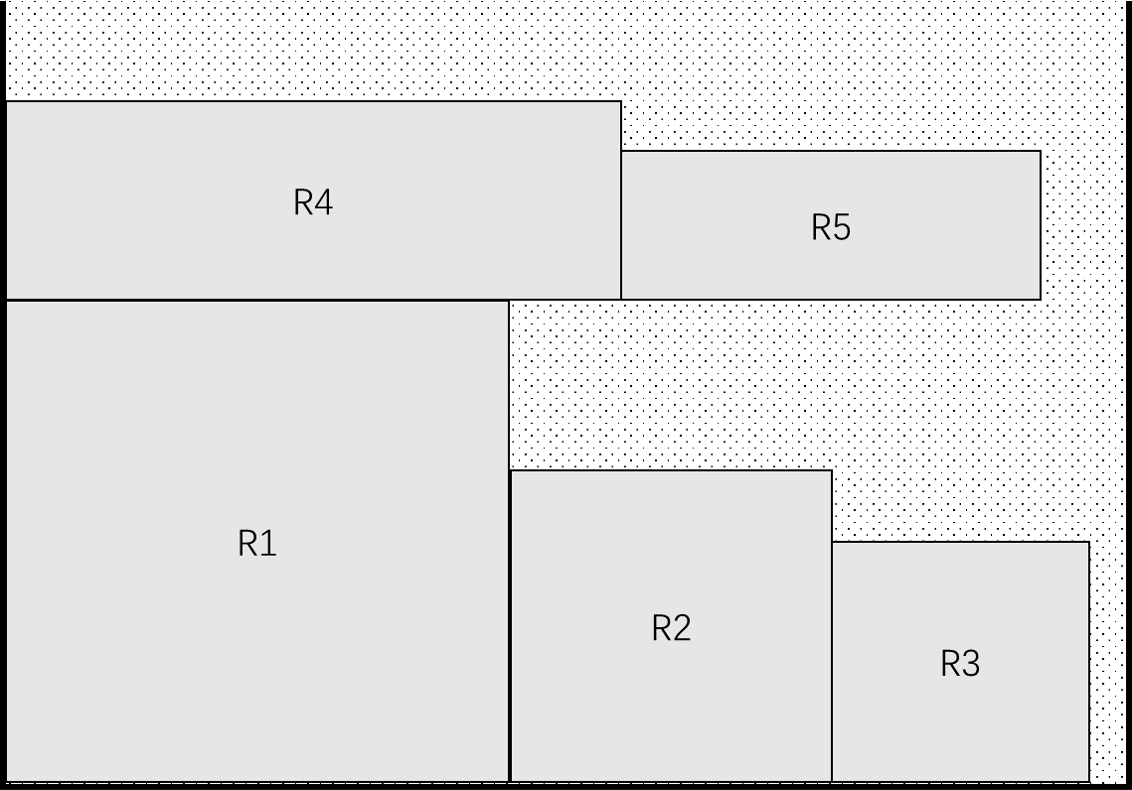
\includegraphics[scale=0.4]{levelbased}
  \caption{Level-Based Packing}
  \label{fig:level-based}
\end{figure}
At first glance, this level-based approach seems wasteful because the space between the level and the rectangle below it is not used. One might think that by putting the rectangle at the lowest-possible place we can achieve a much better result. But as we will show later in the analysis, this new approach will only reduce an additive constant factor which will not affect the algorithm's asymptotic approximation ratio.\par
NFDH and FFDH both are two-dimensional variations of the one-dimensional packing algorithm\cite{johnson1974worst}. They all have a preprocessing procedure to sort all the rectangles with decreasing height. We will introduce both of the 2 algorithms and analyze their approximation ratio in the following subsections.
\subsection{NFDH (Next-Fit Decreasing-Height)}
\paragraph*{Algorithm Description}
NFDH proceed as follows: After we sort all the rectangles with decreasing height. We simply pack rectangles left-justified from left to right on the bottom of the bin (the first level), so the first rectangle is the highest rectangle. When there is no more sufficient width in the current level, we proceed to the next level (a horizontal line on top of the first rectangle in the current level). We just iterate from level to level until we pack all the rectangles.
\paragraph{Performance Analysis}
It may seem that we are wasting space by using the level-based NFDH algorithm, but NFDH has an asymptotic approximation ratio of 2 with an additive factor $h_{max}$ which is the maximum height of all the rectangles and an absolute approximation ratio of 3.
$$NFDH(L) \leq 2*OPT(L) + h_{max}$$
The analysis is shown below, we are normalizing the bin width to be 1 for simplicity.\par
First, we need to introduce some extra symbols for representation. Assume that $x_i$ is the width of the first rectangle at level $i$, $H_i$ is the height of level $i$, $W_i$ is the total weight of level $i$. Then because the first rectangle of level $i+1$ is too big to fit in level $i$, $W_{i} + x_{i+1} \geq 1$ holds. This inequality is used in the proof to relax the result. $A_i$ is the area of level $i$, and $A$ is the total area of all the rectangles. \par
The main idea of the proof is to find a bounded relationship between $A$ and the result $NFDH(L)$. Because the optimal result $OPT(L)$ has to be bigger than the total area $A$, we are able to find an inequality between $NFDH(L)$ and $OPT(L)$. The detailed proof is as follows:
\begin{align*}
  NFDH(L) = \Sigma_{i=1}^{t}H_i  &\leq H_1 + \Sigma_{i=1}^{t-1}H_{i+1}*(W_i + x_{i+1})\\
                & = H_1 + \Sigma_{i=1}^{t-1}(H_{i+1}*W_i + H_{i+1}*x_{i+1})\\
                & \leq H_1 + \Sigma_{i=1}^{t-1}(A_i + A_{i+1})\\
                & \leq H_1 + 2*A\\
                & \leq H_1 + 2*OPT(L)\\
                & = 2*OPT(L) + h_{max} \\
                & \leq 3*OPT(L)
\end{align*}
We will also provide an intuition into the complicated proof: Measuring the approximation ratio for 2D Packing is equivalent to measure how much space we are wasting during packing. For the NFDH algorithm, the wasted space is the empty space between levels. By drawing a horizontal line of height $H_{i+1}$ (which is $\leq H_i$) at level $i$, we are able to partition the wasted space into 2 areas $S_i$ (the empty space above the line) and $T_i$ (the empty space below the line). $S$ has width at most $1$ and height at most $H_i - H_{i+1}$, $T$ has width $1-W_i$ which is smaller that $x_{i+1}$ accoring to the inequality $W_{i} + x_{i+1} \geq 1$, $T$ has height $H_{i+1}$. Then we know that $S_i \leq 1*(H_i - H_{i+1}) = H_i - H_{i+1}$ and $T_i \leq (1 - W_i)*H_{i+1} \leq x_{i+1}*H_{i+1} \leq A_{i+1}$. Then by summing them up, we get $$S = \sum_{i=1}^{t} S_{i} \leq \sum_{i=1}^{t} (H_i - H_{i+1}) = H_1 - H_t \leq H_1 = h_{max}$$ $$T = \sum_{i=1}^{t}T_i \leq \sum_{i=1}^{t}A_{i+1} \leq A$$
Then we are only wasting $A + h_{max}$ spaces, therefore the result: $$NFDH(L) \leq A+S+T \leq 2*A + h_{max} \leq 2*OPT(L) + h_{max}$$
It is also worth mentioning that $S$ (the space between the top of rectangles and the level lines) is the total space wasted by using a level-based approach rather than putting every rectangle at the lowest possible position. Because $S \leq h_{max}$, we know that the level-based approach will only introduce a maximum waste of an additive constant and will not affect the asymptotic approximation ratio.
\subsection{FFDH (First-Fit Decreasing-Height)}
\paragraph*{Algorithm Description}
FFDH basically follows the same procedure as NFDH except that now we can also pack rectangles in the previous level to reuse the wasted space. As shown in figure\ref{fig:ffdhpacking}, $R_6$ will be packed in level 3 for NFDH but is packed in level 1 for FFDH to reuse space. This algorithm definitely performs better than NFDH and has a slightly better asymptotic approximation ratio of 1.7 and an absolute approximation ratio of 2.7. However, it should be noted that FFDH will increase memory usage because it has to track the available width for all the previous levels.
\begin{figure}[htbp]
  \centering
  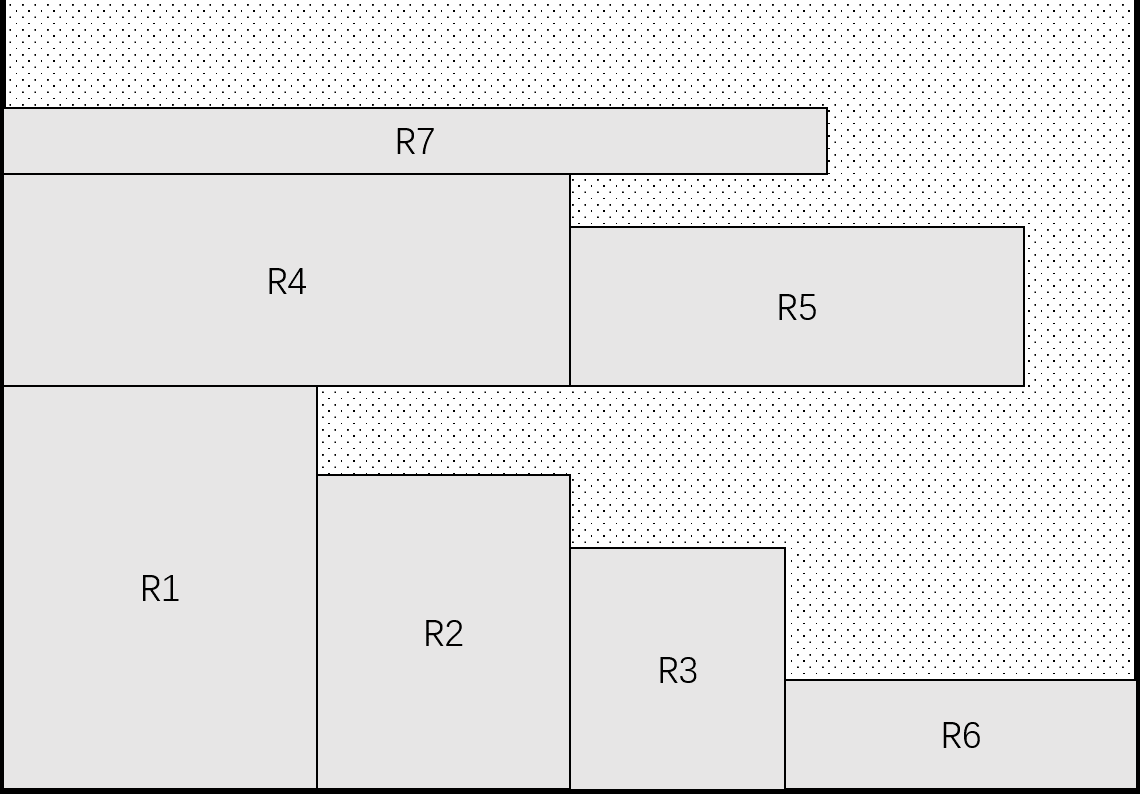
\includegraphics[scale=0.4]{ffdh}
  \caption{FFDH Packing}
  \label{fig:ffdhpacking}
\end{figure}
\paragraph{Performance Analysis}
FFDH has an asymptotic approximation ratio of 1.7 which means that:
$$FFDH(L) \leq 1.7*OPT(L) + h_{max}$$
The main idea of the proof for this approximation ratio is to find an intermediate bound between the total area of rectangles $A$ and $FFDH(L)$. The helper function $W(x)$ used to define the bound in\cite{coffman1980performance} is:
$$ W(x)=\left\{
\begin{aligned}
& \frac{6}{5}x  &   if \text{ } & 0 \leq x \leq \frac{1}{6}\\
& \frac{9}{5}x - \frac{1}{10}  &   if \text{ } & \frac{1}{6} < x \leq \frac{1}{3}\\
& \frac{6}{5}x + \frac{1}{10}  &   if \text{ } & \frac{1}{3} < x \leq \frac{1}{2}\\
& \frac{6}{5}x + \frac{2}{5}  &   if \text{ } & \frac{1}{2} < x \leq 1
\end{aligned}
\right.
$$
And it is shown in\cite{garey1976resource} that no collection of $x$ summing to 1 can have $W(x)$ sum to more than 1.7. Coffman's paper\cite{coffman1980performance} uses this helper function to bound the optimal result by split the optimal solution into pieces\cite{coffman1980performance}. The intermediate bound is as follows:
$$I = \sum_{r \in R}h(r)*W(w(r)) \leq 1.7*OPT(L)$$
The paper also forms an inequality between the result $FFDH(L)$ and $I$:
$$I \geq FFDH(L) - h_{max}$$
The proof for this inequality is very complicated so we will not dig into that in this paper, you can always read the full comprehensive proof in\cite{coffman1980performance}. Then by combining the two inequalities, we can get the relationship between $FFDH(L)$ and $OPT(L)$:
$$FFDH(L) \leq I + h_{max} \leq 1.7*OPT(L) + h_{max} \leq 2.7*OPT(L)$$
Then we can conclude that $FFDH$ has an asymptotic approximation ratio of 1.7 and an absolute approximation ratio of 2.7.\par
Now we have looked at the 2 heuristic intuitive approximation algorithms with an absolute approximation ratio of 3 and 2.7, one may wonder is it possible to get a tighter bound using a different approach? The answer is yes, as we will show in the next section, we can get a much better absolute approximation ratio of 2 using a constraints-driven approach.
\section{Steinberg's Algorithm}
\par In this section we introduce a more advanced approximation algorithm designed by \cite{steinberg1997strip}. Instead of heuristically packing every rectangle and output the height as result, Steinberg gave a more specific bound on the height $\hat{h}$ of the bin, with which a valid packing can be found easily. This is guaranteed by the following theorem.
\paragraph{Steinberg's Theorem} If the following inequalities hold
\begin{eqnarray}
	a_M &= \max_{1\leq i\leq n} a_i \\
	b_M &= \max_{1\leq i\leq n} b_i \\
\end{eqnarray}
\bibliographystyle{acm}
\bibliography{paper}
\end{document}
\endinput
